\documentclass{ctexart}
\usepackage{ctex}
\usepackage{graphicx}
\usepackage{amsmath}
\usepackage{amsfonts}
\usepackage{listings}

\graphicspath{{figures/}}

\title{VP树}
\author{Mr Wu}
\date{\today}

\begin{document}
	\maketitle
	\section{介绍}
	VP树是更具体的度量树,可以有效划分$ n $维度量空间中的数据。VP树在执行范围查询时有优势。
	
	考虑二维平面上一个包含1000个点的数据集。VP树的每个结点包含以下五方面信息:
	
	数据:它包含的数据点列表;
	
	vp:从数据中选取的一个优势点;
	
	mu:定义这个结点范围的一个半径值;
	
	inside:左子树;
	
	outside:右子树。
	
	\section{创建}
	现在开始创建根结点。根结点的数据包含所有数据点。选择一个好的vp可以直接影响树的效率,但为了方便起见,我们随机选取一个数据点。
	
	选择好vp之后,开始计算mu,使得一半数据在半径范围之内。
	
	接下来再细分数据点。创建左子树,包含所有圆内的数据点;创建右子树,包含所有圆外的点。如此递归,直到子树中不包含数据点。对于1000个点的数据集,只需要划分9次。
	
	\section{分析}
	每一层递归将原始问题划分为两个相同规模的子问题。在每个结点,必须计算出结点所包含数据的中位数,用来得到mu值。对于每一层,这个操作的复杂度为$ O(n) $。
	
	树的深度为$ O(logn) $,因此创建一个VP树的总复杂度为$ O(nlogn) $。
	
	\section{搜索}
	搜索目标是通过查询尽可能少的结点来找到查询点的最近邻。
	
	考虑一个半径为tau的以查询点为圆心的圆,包含它的所有最近邻。假设要找k近邻,则tau会包含最近的k个数据点。
	
	考虑$ k=3 $的情况:
	14个数据点(黑点),查询点(红点),vp(蓝点),mu(蓝圈),tau(红圈)。
	
	情形1:
	
	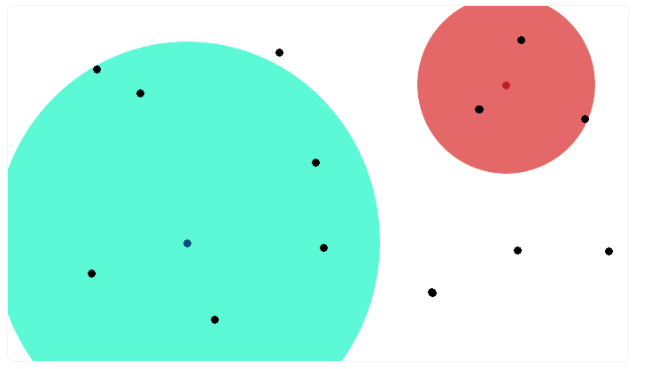
\includegraphics[scale=0.5]{case1}
	
	注意到tau完全在mu之外,也就是查询点的最近邻全在右子树中。所以可以剪去左子树,工作量减半。
	
	情形2:
	
	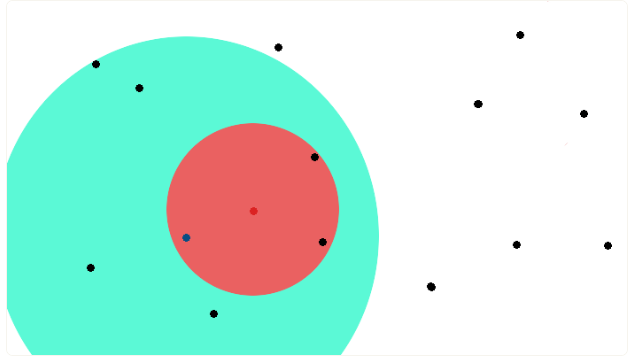
\includegraphics[scale=0.5]{case2}
	
	与情形1正好相反,可以剪去右子树。
	
	情形3:
	
	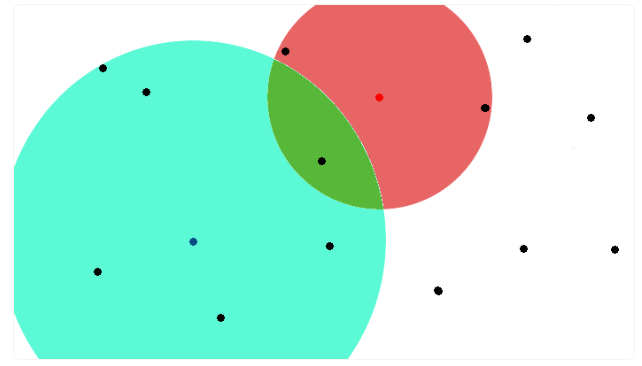
\includegraphics[scale=0.5]{case3}
	
	此时tau和mu相交,无法剪枝,必须搜索左右子树。
	
	搜索树的时候,可以把tau看成查询点周围感兴趣的区域。从无穷大开始,通过剪去感兴趣区域之外的点,来逐步缩小tau。
	\section{实现以及复杂度分析}
	
\end{document}